% Exercise Template
% A LaTeX document for بخش چهارم: چالش پیاده‌سازی نیمه‌پیشرفته
% By: Maryam soofi

\documentclass[12pt]{exam}

\usepackage{setspace}
\usepackage{listings}
\usepackage{xcolor}
\usepackage{xepersian}

% Define colors
\definecolor{codegreen}{rgb}{0,0.6,0}
\definecolor{codegray}{rgb}{0.5,0.5,0.5}
\definecolor{codepurple}{rgb}{0.58,0,0.82}
\definecolor{backcolour}{rgb}{0.95,0.95,0.92}

% Configure listings style
\lstdefinestyle{mystyle}{
	backgroundcolor=\color{backcolour},   
	commentstyle=\color{codegreen},
	keywordstyle=\color{magenta},
	numberstyle=\tiny\color{codegray},
	stringstyle=\color{codepurple},
	basicstyle=\ttfamily\footnotesize\setLTR,
	breakatwhitespace=true,
	breaklines=true,
	captionpos=top,
	keepspaces=true,
	numbers=left,
	numbersep=5pt,
	showspaces=false,
	showstringspaces=false,
	showtabs=false,
	tabsize=2,
	frame=single,
	abovecaptionskip=5pt,
	belowcaptionskip=5pt,
}

\lstset{style=mystyle}
\renewcommand{\lstlistingname}{برنامه}
\usepackage{graphicx,subfigure,wrapfig}
\usepackage{float}
\usepackage{multirow}
\usepackage{pgf-pie}
\usepackage{etoolbox}
\usepackage[margin=20mm]{geometry}
\usepackage{hyperref}
\hypersetup{
	colorlinks=true,
	linkcolor=blue,
	filecolor=magenta,
	urlcolor=cyan,
	pdftitle={بخش چهارم: چالش پیاده‌سازی نیمه‌پیشرفته},
	pdfpagemode=FullScreen,
}
\settextfont{XB Niloofar}

\begin{document}
	
	\vspace{1em}
	
	در این بخش شما را به چالش می‌کشد تا با پیاده‌سازی تکنیک‌های پیشرفته‌تر، عملکرد و درک خود از شبکه‌های عصبی را عمیق‌تر کنید.
	
	\begin{questions}
		
		% Task 1
		\question
		\textbf{پیاده‌سازی الگوریتم بهینه‌ساز مومنتوم و مقایسه سرعت همگرایی}
		
		الگوریتم بهینه‌ساز Momentum را پیاده‌سازی کنید و سرعت همگرایی آن را با گرادیان کاهشی استاندارد در بخش 3 مقایسه نمایید. نمودار فاصله تا بهینگی یا مقدار تابع هزینه در هر دوره را رسم کنید.

		
		\lstinputlisting[language=Python, caption=پیاده‌سازی \lr{Momentum}]{./scripts/momentum\_optimizer.py}
		
		% Task 2
		\question
		\textbf{رسم نمودارهای زیان و دقت}
		
		نمودارهای زیان (loss) و دقت (accuracy) آموزش را در طول دوره‌ها برای بخش 3 رسم کنید. در صورت پیاده‌سازی تقسیم اعتبارسنجی \lr{(cross-validation split)} نمودارهای زیان و دقت اعتبارسنجی را نیز اضافه نمایید.
		
		\lstinputlisting[language=Python, caption= رسم نمودار زیان و دقت آموزش و اعتبارسنجی]{./scripts/plot\_metrics.py}
		
		\begin{figure}[H]
			\centering
			\subfigure[نمودار زیان (Loss)]{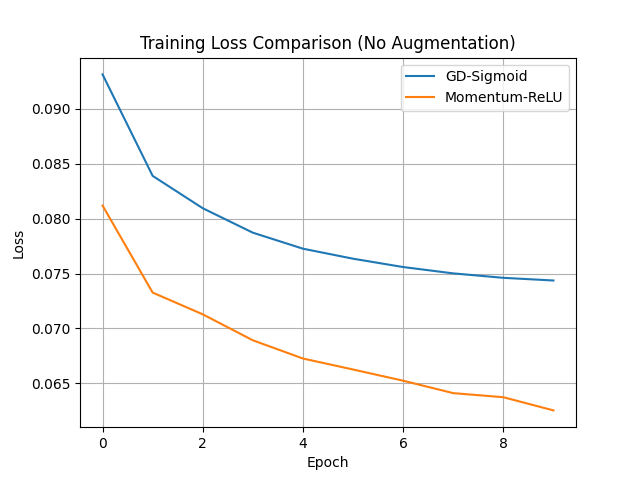
\includegraphics[width=0.45\textwidth]{./figures/loss.png}}\quad
			\subfigure[نمودار دقت (Accuracy)]{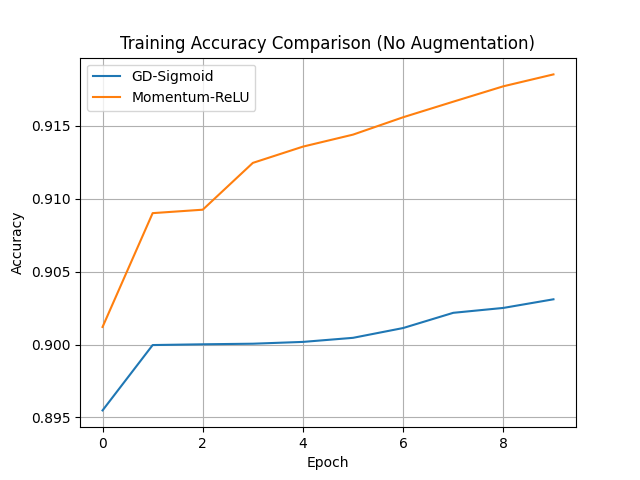
\includegraphics[width=0.45\textwidth]{./figures/accuracy.png}}  
			\caption{مقایسهٔ زیان و دقت آموزش و اعتبارسنجی در طول دوره‌ها}
			\label{fig:loss_acc_plots}
		\end{figure}
		
		% Task 3
		\question
		\textbf{استفاده از تابع فعال‌سازی ReLU و مقایسه با سیگموئید}
		
		در لایه‌های پنهان شبکه خود از تابع ReLU استفاده کنید و عملکرد آن را با سیگموئید مقایسه نمایید. مقداردهی اولیه وزن‌ها را با \lr{He Initialization} تنظیم کنید.

		
		\lstinputlisting[language=Python, caption= مقداردهی اولیه‌ی \lr{Relu}]{./scripts/relu\_he\_initialization.py}
		
		% Task 4
		\question
		\textbf{ساخت کلاس مدولار NeuralNetwork()}
		
		یک کلاس مدولار \verb|NeuralNetwork()| بسازید که امکانات زیر را فراهم کند:
		\begin{itemize}
			\item تعریف تعداد دلخواه لایه با اندازه‌های مشخص
			\item انتخاب توابع فعال‌سازی مختلف برای هر لایه \lr{(sigmoid, ReLU, tanh, SGD, momentum, Adam)}
			\item پیاده‌سازی بهینه‌سازهای مختلف
		\end{itemize}
		
		
		\lstinputlisting[language=Python, caption= کلاس \lr{Neural Network}]{./scripts/modular\_nn.py}
		
		% Task 5
		\question
		\textbf{آموزش و مقایسه مدل‌ها}
		
		مدل طبقه‌بندی خود را با انتخاب ترکیب‌های مختلف از موارد بالا آموزش دهید و نتایج آن‌ها را مقایسه نمایید. می‌توانید جدول یا نمودار مقایسه دقت و زمان آموزش ایجاد کنید.
		

		\lstinputlisting[language=Python, caption= آموزش و مقایسه مدل‌ها]{./scripts/compare\_models.py}
		
	\end{questions}
	
\end{document}
